\documentclass[letterpaper, 12pt]{article}


\usepackage{cmjStyle-pdftex} %use CMJ style
\usepackage{natbib} %natbib package, necessary for customized cmj BibTeX style
\bibpunct{(}{)}{;}{a}{}{,} %adapt style of references in text

\doublespacing


\raggedright % use this to remove spacing and hyphenation oddities
%\setlength{\parindent}{0} % first para indent?
\setlength{\parskip}{2ex}
\parindent 24pt
\urlstyle{same} % make url tags have the same font
\setcounter{secnumdepth}{-1} % remove section numbering

\usepackage{ifpdf}

\DeclareGraphicsExtensions{.pdf,.png,.jpg}
\graphicspath{{../fig/}}


%% The package endfloat moves all floats (figures, tables...) to the end of the paper, as required for the final version of a CMJ paper.
%% Leave this package commented out for initial submission, but uncomment it for final version. 

 % \usepackage{endfloat}

\usepackage{microtype}

%---Document----------
\begin{document}

{\cmjTitle 	Computation as material: (meta) live coding experiences}
\vspace*{24pt}

% (In the initial submission, omit all the following author information to ensure anonymity during peer review.)

%author - name
% {\cmjAuthor Till Bovermann}
% %author - address
% \newline
% \begin{cmjAuthorAddress}
% 	Media Lab Helsinki, Department of Media\\
% 	Aalto University\\
% 	H\"ameentie 135 c\\
% 	00560 Helsinki, Finland\\
% 	till.bovermann@aalto.fi
% \end{cmjAuthorAddress}
% 
% \vspace*{24pt}
% {\cmjAuthorPhone +358 (50) 5296398}
% \vspace*{24pt}
% 
% %author - name
% {\cmjAuthor Dave Griffiths}
% %author - address
% \newline
% \begin{cmjAuthorAddress}
% 	FoAM\\
% 	Koolmijnenkaai 30-34\\
% 	1080 Brussels\\
% 	Belgium\\
% 	dave@fo.am
% \end{cmjAuthorAddress}
% 
% \vspace*{24pt}
% {\cmjAuthorPhone +32 2 5135928}
% \vspace*{24pt}


% TODO write abstract
\begin{abstract}
How can low-level computation sound and how can it be integrated into livecoding practices?
This paper gives insights into three years of artistic research and performance practice with Betablocker, an imaginary CPU architecture, specifically designed and implemented for livecoding purposes.
It covers the themes of algorithmic composition, sound generation, genetic programming and autonomous coding in the light of self-manipulating code and artistic research practice.
\end{abstract}

% TODO write discussion
% TODO collecting cites
% TODO Daves performance part

% \section{}

% + how people imagine computation now (scary stuff) (Dave)

Computation is odd. 
In fact in many ways it's one of the strangest things we have discovered, and 77 years on we continue to fail to fully grasp it's behaviour.
And so, we struggle to keep unseen ramifications of our decisions under control. Faced with such a strange and yet essential beast, the only sane strategy is to try and tame it. 
The field of software engineering, the field emerged around the topic of computation, is littered with concepts such as regression testing, type checking, white rooms, sandboxing, contracts, and encapsulation -- all attempts to cope with the fact that we fail to naturally understand how a mundane machine of sufficient complexity will act when it is programmed by a human.

Livecoders look this beast straight in the eyes. 
When a livecoding performer takes to the stage and projects her screen, she invites us to join her in attempting to understand this intricate dance between human and machine. 

% livecoding is manifold: performance, research practice
Beyond performance practice, livecoding is a broad field that can be viewed from many different angles.
From rehearsed public performances, collaborative improvisations and individual sound explorations, to it's utilisation as a method in science, it has been utilised in a manifold of applications.
All these derivations of the original theme share elements of live coding as they are featured in the Toplap manifesto draft.\footnote{\url{http://toplap.org/wiki/ManifestoDraft}}
Livecoding attempts to treat computation as a material on it's own terms, to pick it up and feel what shapes it has.

Based on this ground, we introduce Betablocker, an approach to livecoding which has brought to light many different strategies for presenting computation as a tangible material -- and it does this by making this process as much part of the performance as the code that describes it.
Built around this element is a variety of applications for testing, exploring and performing scientific as well as artistic investigations.

% Three levels: (a) technology, (b) unfolding as performance/research practice/method (conceptual and descriptive) and (c) aesthetic qualities.

This paper collects experiences, challenges and insights gathered by the two authors over the course of 3 years while they designed imaginary CPU architectures and investigated the combination of established as well as emerging live coding techniques.
Central to the work presented here is the use of livecoding cultures, performance contexts and exploration strategies in order to gain understandings of behaviour emerging from simple instructions sets when given self-alteration abilities. 
This leads us towards a kind of second-order livecoding where, starting with nothing, programs written a few minutes ago interact and interfere with the programming of subsequent programs or even write programs all of their own.

\parskip 18pt

\section{BetaBlocker core technology} 
\label{sec:betablocker_core}

% describing the theoretical background and implementation (switch statement etc.)

The core of all investigations described in this paper is the Betablocker engine, is a highly simplified multithreaded virtual machine.

The BetaBlocker engine consists of 
(a) a \emph{heap} with  $2^8 = 256$ addressable slots to store an 8bit value (a byte), 
(b) an \emph{instruction table} linking a byte to an atomic instruction, and
(c) a number of independent \emph{threads}, each with a 
	(ca) an 8bit \emph{program counter} (\texttt{pC}) pointing to an address in the heap, and (cb) a \emph{stack} of eight bytes.
The state vector consisting of a heap, a stack and a program counter sufficiently represents the state of a Betablocker engine.

The heap is where all data is stored. 
Following \emph{von Neumann architecture} \citep*{von-neumann1993-fir}, Betablocker computation does not make any distinction between a program (i.e., an instruction set) and data (i.e., data on which the program operates). 
The notions of code, data and program are therefore synonyms, however they represent semantical meaning rather than systematical/structural meaning.
Particular attention has to be given to the fact that, although a specific part of data stored on Betablocker's heap is meant to be a program, by definition the possibility exists that it is altered (e.g., by a separate process running independently on the same heap or even by itself).
In reverse, a critical differentiation with other virtual machines (eg. Java VM, the .NET CLR) is therefore that every possible combination of values is a valid program and that each of these values is interpreted either as an instruction, an address, or a data item. 


\begin{figure}
	\centering
		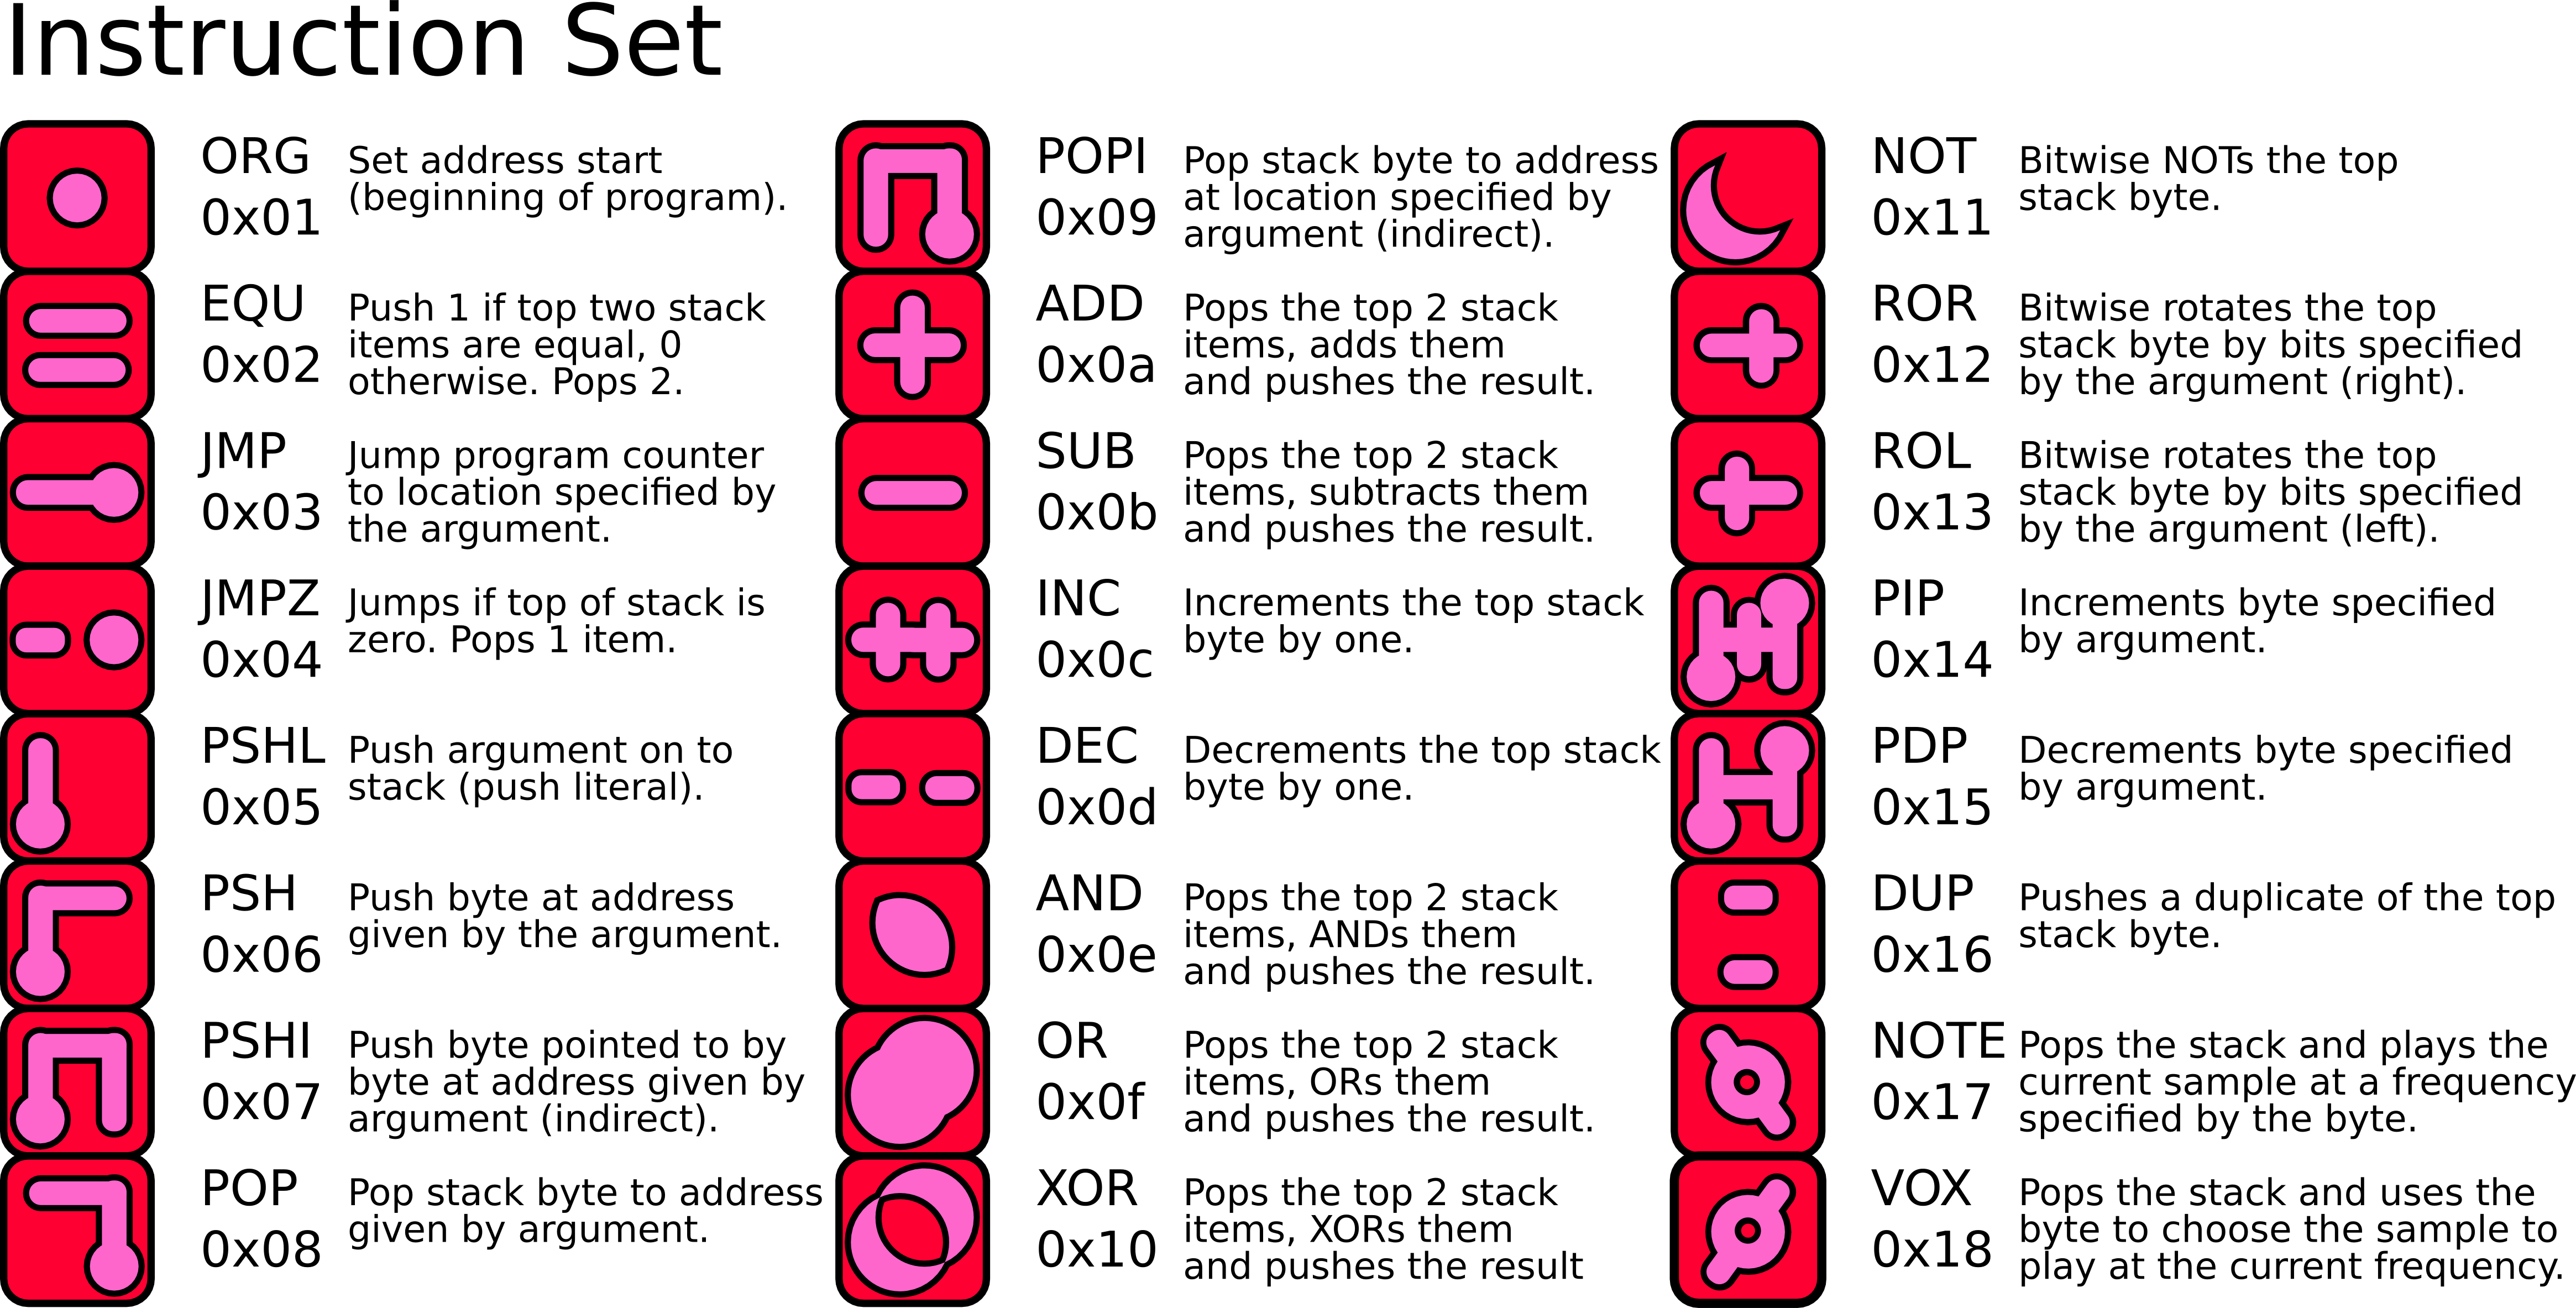
\includegraphics[width=13cm]{bbds-legend}
	\caption{Betablocker instructions.}
	\label{fig:fig_bbds-legend}
\end{figure}


% instruction set
Regarding the instruction table, we differentiate between the core set which consists of 22 distinct instructions and various extensions to this set, which, depending on the actual application, introduce features like playing a note (\texttt{NOTE}) or copying information to the output pins of an AVR chip (\texttt{OUT}).
An overview of the instructions is given in Figure~\ref{fig:fig_bbds-legend}.
As there is no instructions, interrupts or error states telling the engine to halt, programs will continue to run (possibly in infinite loops) until externally terminated.
However, they will eventually converge into a (possibly complex) stable state.

% thread
A thread executes code stored on the heap. 
Its program counter $pC$ stores the current position (i.e., the instruction it is currently evaluating).
The stack serves as a temporary private storage for a thread, not addressable by other threads. 
It is accessed by either \emph{popping} an item from the stack to an adress or the indirect location specified by an address (e.g.~\texttt{POP}~\texttt{POPI}), or pushing a value to the stack in immediate/literal, address or indirect variants  (e.g.~\texttt{PSHL},~\texttt{PSH},~\texttt{PSHI}). All mathematical processes operate using the stack rather than using registers, so the resulting language is close to Forth.
% TODO: cite Forth


\parskip 18pt

\section{Background and historical context} 
\label{sec:background}

% musical and computational

Betablocker first came to life as an attempt at a game pad programmable live coding system in fluxus.\footnote{
% TODO: add fluxus link
(Fluxus link)
} 
It was inspired by a discussion on the TOPLAP mailing list about virtual machines, and by games such as \emph{Mr Driller} in terms of colourful blocks interacting with each other and setting up chain reactions as a game mechanic.\footnote{
% TODO: add Mr Driller link
(Mr Driller link)
}
 
Core Wars\footnote{
% TODO: add Code Wars link
(Code Wars link)
}, a game where programmer/contestants write simple programs that battle to gain memory footprint over each other was also an important inspiration, both in terms of domain specific low level languages, and imaginary hardware.

From a musical point of view, Betablocker can be viewed as a tool for algorithmic composition \citep*{maurer1999-a-b} and simultaneous sonification and visualisation of the process.
Also, it is inspired by nonlinear and stochastic synthesis techniques as described by Xenakis \citep*{Xenakis:1971, luque2009-the}.



\parskip 18pt

\section{Livecoding philosophy and aesthetic findings}
\label{sec:distinct_character}

% \subsection{Computational features} 
% \label{sub:computational_features}

% a particular take on livecoding
% grounding it in process rather than code
% and
% computation as material

BetaBlocker is distinct to other approaches of computational machines in several aspects:
In the design of Betablocker, the ability to observe computational behaviour was an essential goal, whereas the result of the computation (and therefore process optimisation) played a minor role.  
Furthermore, Betablocker is implemented as a software emulation and can be modified easily.
This allows for its alteration regarding introspection (by adding probes) and customisation (by altering the instruction set).
Last not least, compared to common microprocessor architectures such as the x86\footnote{\url{http://en.wikipedia.org/wiki/X86}} or even RISC\footnote{\url{http://en.wikipedia.org/wiki/Reduced_instruction_set_computing}} microcontrollers such as AVR\footnote{\url{http://en.wikipedia.org/wiki/Atmel_AVR}}, Betablocker's architecture is extremely simplistic.
Operational complexity arises from the induced data and its processing rather than from the system's architectural features.

The character of Betablocker influences not only the sonic results of a livecoding session but also its overall structuring.
Due to its potential process complexity, it is e.g. possible to start with a blank page\footnote{As proposed in the TOPLAP Manifesto draft published at \url{http://toplap.org/wiki/ManifestoDraft}.}
and build complicated patterns which remain controllable as the next step.

We describe our findings and explorations with regard to Betablocker in the next paragraphs and give insights on how its behaviour influenced our livecoding sessions.
As we used Betablocker mainly in two perceptional contrasting settings, \emph{rhythmic}, which slowed down processing in order to percieve it and \emph{sonic}, speeding up processing in order to hear it's sonic properties directly, we differentiate in the following between Betablocker/Rhythm and Betablocker/Audio.

\parskip 18pt

\subsection{Slow computing -- Betablocker/Rhythm}
\label{sub:slow_computing}
%  describing the nintendoDS part of the implementation

% TODO: more detail, also technical level... graphical interface, why you chose the grid gui etc.

Betablocker/Rhythm (the Fluxus and Gameboy DS version) makes computation tangible by slowing down processes by many orders of magnitude compared to typical scenarios. 
The smallest musical loop in Betablocker/Rhythm is 3 instructions long -- push a value onto the stack (\texttt{PSH, 123}), play it as a note (\texttt{NOTE}), jump back to start (\texttt{JMP 0}). 
In order to play this at 120 BPM it will need to run at 6 cycles per second, the machine I am typing on peaks at $2.8*10^9$ cycles per second, which is 466 million times faster than Betablocker/Slow. This makes computation audible as techno music, and simultaneously visible as the thread's positions are displayed on the livecoding interface synced with the audio along with the entire heap's memory contents.

Performing with Betablocker/Rhythm consists of starting with empty memory and manually entering programs byte by byte that modify themselves and each other. Bytes used as address locations are visualised literally as pointers - arrows indicating the address in memory they are referencing. 
Eventually the quantity of self replicating fork bombs, sequencers interpreting memory as percussion synth triggers and programs busily reversing the contents of memory reaches a level where the performer is confronted with a kind of 'Turing soup' which is writing it's own code. 
At this point the decision is whether to take advantage of this situation or rather gain control over it.
Taking advantage of it involves looking for interesting sections of code that emerge and manually modifying them, while the best strategy for getting back control is attempting to find a space to write a program that gradually clears memory so you can start again. 
In most successful performances both options were taken over the course of the concert.

It is this gradual cessation of control, with immediacy and totality of the understanding (or at very least display) of the machine that sets this apart from traditional livecoding performance, where the high level description of a process is the only connection between the audience and performer and process creating the music they hear.

In order to further illustrate the kinds of programs and livecoding strategies, we list concrete 'code patterns' which are used in common live coding situations.

Firstly, a program which will play all the sounds in a sound bank at all frequencies available. 
Multiple threads can be issued to play this program at the same time to provide more complexity. 
Values interpreted as pointers are visualised as arrows:
% TODO: figures are floats and not inline. Fix ":"

\begin{figure}[H]
	\centering
		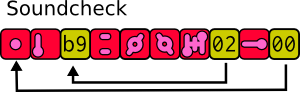
\includegraphics[width=8cm]{bbds-sndchk1}
	\caption{Sound check}
	\label{fig:fig_bbds-sndchk1}
\end{figure}

In Betablocker/Rhythm the beat is always locked to the instruction cycle, so faster melodies or beats are a matter of optimisation. Fast inner loop programs can be used for playing sounds while another slower program modifies the first by overwriting parts of it while it's running, as in this example. 

\begin{figure}[H]
	\centering
		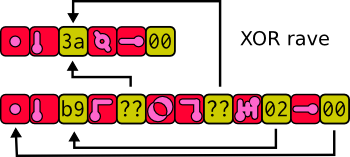
\includegraphics[width=8cm]{bbds-xorrave}
	\caption{XOR rave}
	\label{fig:fig_bbds-xorrave}
\end{figure}

The following programs are both 16 bytes long, and require 3 concurrent threads to be running over different parts of the program. From left to right, the first thread loads an immediate byte and plays it as a sound repeatedly, the second one increments the byte that the first is loading, and the third periodically resets the byte to a constant value.
 
\begin{figure}[H]
	\centering
	% TODO: caption
		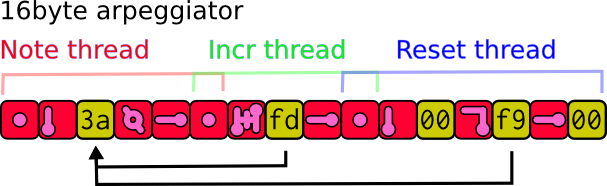
\includegraphics[width=10cm]{bbds-arp}
	\caption{Simple arpeggiator}
	\label{fig:fig_bbds-arp}
\end{figure}

The first example simply plays the byte as a note - resulting in an arpeggiator style sound. After writing the code, the performer can change the speed of each of the three threads to get more variety. For example, the slower the resetting thread runs, the longer the pattern will be before it repeats.

\begin{figure}[H]
	\centering
		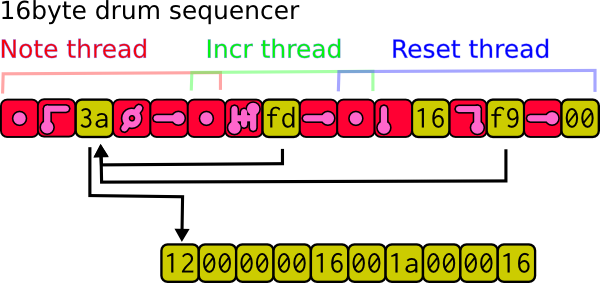
\includegraphics[width=10cm]{bbds-seq}
	\caption{Sequencer}
	\label{fig:fig_bbds-seq}
\end{figure}

The second example is very similar, but is slightly modified to play a sequence of different sounds rather than notes, in order to become a percussion sequencer. The second instruction is changed from a "push literal" to a "push contents of address" which results in the program playing a part of memory as a sequence. We can control the start address location with the reset byte, write directly to this part of memory, and fiddle with the other thread's speed to get even more complexity.

Other types of program alter the memory rather than focus on sound. 
For example given two addresses, a program may increment one and decrement the other copying bytes from the source to the destination, which results in the entire CPU memory to be reversed. 
Another type of program is might be called "self replicating fork bomb": It copies its code to a other locations and therefore captures parallel threads of execution.

\parskip 18pt

\subsubsection{Use of Genetic Algorithms as creative augmentation in livecoding} % (fold)
\label{sub:genetic_programming}

The same features that makes the Betablocker approach suitable for exploratory artistic and musical applications (lack of error states and code/data isomorphism) also make it a highly convenient environment for employing evolutionary strategies.

% TODO: cite genetic algorithms
The use of Genetic Algorithms in livecoding presents different purposes to producing efficient and novel solutions to problems specified by a fitness function. In the case of Betablocker/Rhythm the desire initially to use genetic algorithm's arose from the need to learn new, optimal coding patterns for use in livecoding performances, a way of escaping a feeling of being 'stuck in a creative rut'. The use of a genetic algorithm in this case it to provide \emph{new ideas for artistic use} - not final programs for their own sake.

The success of an algorithm used for livecoding is to some extent how easy it is to change, how malleable it is, and one of the features of evolutionary strategy is that programs are automatically converged on that may present extremely unorthodox approaches - especially when optimisation is linked to fitness criteria and architectures are used where self modification is possible. In this case we use want to unpick these approaches in order to employ them musically in hand written code.

In a genetic algorithm, in order to select promising individual programs from a population, we need a way to judge fitness. In this application we are creating lists of note numbers, and in order to create a fitness metric we favour patterns that have unique notes (to avoid repetition) but also look for a rhythmic nature by measuring them with this function:

\begin{Verbatim}[fontfamily=courier, xleftmargin=\parindent]
(defn freq [l n]
  (defn _ [c]
    (cond
     (>= (+ c n) (count l)) 0
     (= (nth l c) (nth l (+ c n))) (+ 1 (_ (+ c 1)))
     :else (_ (+ c 1))))
  (_ 0))
\end{Verbatim}

Which looks for repeating values spaced apart by "n" positions, so:

\begin{Verbatim}[fontfamily=courier, xleftmargin=\parindent]
(freq '(100 1 2 3 100 4 5 6 100 7 8 9 100) 4) 
\end{Verbatim}

Returns 3, as it finds 3 pairs of equal values (100) distanced by the specified 4 positions.

With this fitness function:

\begin{Verbatim}[fontfamily=courier, xleftmargin=\parindent]
(+ (* 50 (count (num-unique res))) ; unique notes are very good
   (freq res 4) ; equal notes every 4 beats are good
   (freq res 6)) ; equal notes every 6 beats are good
\end{Verbatim}

We favour rhythmic components of 4 or 6 beats and boost the uniqueness score by multiplying it by 50. Here is a resulting evolved individual 16 byte program:

\begin{figure}[H]
	\centering
		
\includegraphics[width=10cm]{evolved}
	\caption{Evolved program}
	\label{fig:evolved}
\end{figure}

This program creates a pattern from four separate sources:
 (a) a descending scale using the stack to store the current position,
 (b) a rising scale by self modifying address 12 (the 0 in \texttt{PSHL 0}),
 (c) playing it's own code as a pattern of notes by using address 12 as a pointer, and
 (d) playing the bitwise \texttt{NOT} of it's own code at the same time.
% 
% \begin{enumerate}
% \item A descending scale using the stack to store the current position.
% \item A rising scale by self modifying address 12 (the 0 in \texttt{PSHL 0}).
% \item Playing it's own code as a pattern of notes by using address 12 as a pointer.
% \item Playing the bitwise \texttt{NOT} of it's own code at the same time.
% \end{enumerate}
% 
The result: \texttt{0 0 232 255 23 1 232 254 13 2 242 253 22 3 233 252 7 4 248 251 12 5 243 250 17 6 238 249 20 7 235 248 12 8} scores poorly for its rhythmic patterns, but it is probable that this surprising local maxima was found by the early influence of the rhythmic fitness criteria on its ancestor populations. 

The evolved programs provided many new ideas used for livecoding performances,  including self playing programs like the one above, greater use of stack (evolved programs showed less reliance on storing values on the heap, leading to more robust programs) and more importantly, a general reappraisal of the potential scope of programs possible in this restricted framework.

Following this work, Betablocker was ported as \emph{Spork Factory} to the ATtiny processor as part of an ongoing investigation of physical, livecodable objects and robots. 
The instruction set was extended by \texttt{IN} and \texttt{OUT} instructions for accessing the pins of the microcontroller. 
This enabled audio programs to be evolved for the processor, using FFT analysis on the resulting sounds as the data to provide fitness metrics for.

% In a second attempt, Spork Factory, an additionally introduced instruction (\texttt{OUT}) writes out the topmost value on the stack to the pins of a microcontroller to be converted to sound.
% In difference to the probing approach, this feature decouples sound output from computation, however requires faster execution rates to produce the same output.\footnote{Each instruction \texttt{I} that changes the stack has to be replaced by \texttt{[I, DUP, OUT]}}
% In the next paragraphs, we will describe the implementation and implications of the first attempt.



\parskip 18pt

\subsection{Sound computing -- Betablocker/Audio} 
\label{sub:sound_computing}
%   + SuperCollider (Till)

% bytecode synthesis
One goal of the investigation into Betablocker was to gain new insights into the aesthetics of typical data processing.
How dynamic is the behaviour of a chip when it runs an algorithm?
How does computation sound like and is the variety of programs reflected in a diversity of sounds?
To get answers to these questions, we facilitated the method of introducing \emph{pointsOfTouch} for sonification-supported research \citep{bovermann2011-the}.
Just as it is possible to probe hardware circuitry with e.g. the \emph{Audio Sniffer}\footnote{\url{http://www.openmusiclabs.com/projects/audio-sniffer/}}, we intended to probe Betablocker engines while executing their heaps.

To be able to capture signals in the audible range, the Betablocker/Audio variation runs at rates around typical audio sampling rates.
Because of the intention to probe an otherwise independent system, no separate instructions or other structural enhancements that would influence its computational behaviour were introduced to the Betablocker engine.
Instead, we added \emph{pointsOfTouch} to meaningful parts like the stack and the program counter.

The implementation of Betablocker/Audio was done in the SuperCollider programming environment.\footnote{The source code is available as a plugin to Supercollider from  \url{https://github.com/supercollider/sc3-plugins}.}
To facilitate typical usage, we decided to provide two different interfaces: a demand-rate UGen (\texttt{DetaBlockerBuf}) exposing the topmost value of the stack by means of SuperCollider's demand chain implementation, and a multi-out version (\texttt{BBlockerBuf}) that exposes the position of the program counter as well as  the complete stack.
A basic example on how they can be accessed is given in the following listings.\footnote{
It is assumed that the heap to be operated on is pre-loaded into a Buffer object.
}
By applying a \texttt{LeakDC} operation to the stack values, DC offsets that could harm the speaker system are removed.


\begin{Verbatim}[fontfamily=courier, xleftmargin=\parindent]
x = { // BBlockerBuf example
	var signal = Demand.ar(
	  Impulse.ar('bbRate'.kr(22100)), 
	  'reset'.tr(0),
	  DetaBlockerBuf('heapBuf'.kr(0))
	);
	LeakDC.ar(signal);
}.play;
\end{Verbatim}

\begin{Verbatim}[fontfamily=courier, xleftmargin=\parindent]
x = { // BBlockerBuf example
	var pC, stack;
	#pC ... stack = BBlockerBuf.ar('bbRate'.kr(22100), 
		'heapBuf'.kr(0), 'startpoint'.kr(0));
	stack = LeakDC.ar(stack);
	 // use information on program counter to place sound output
	Splay.ar(stack, spread: 0.1, center: pC);
}.play;
\end{Verbatim}

\parskip 18pt

\subsubsection{Noise aesthetics -- on texture and rhythm} 
\label{sub:noise_aesthetics}

% playing random instruction sequences vs. "conscious" programming
Although the system is deterministic, i.e., its outcome can be calculated supposed its state is known.
Due to it's complexity a valid and, as it turned out, fruitful approach is to work with randomness and empirical observations rather than with analytical approaches.

% analysis/findings
To investigate into this, we implemented a cluster generator for synthesising Betablocker operations of randomly generated heaps:
\begin{Verbatim}[fontfamily=courier, xleftmargin=\parindent]
{var srcs = ({BBlockerBuf.ar(
    s.sampleRate * 0.5, 
    BBlockerProgram({rrand(0, 24)}!256).makeLocalBuf
  )[1]}!20);
  Splay.ar(srcs.collect{|src| LeakDC.ar(src)}, 1, 0.4);
}.play
\end{Verbatim}
After extensive listening, we found out that they often sound like airily high-pitched and infinitely sustained sound clouds, broken up occasionally by a rhythmical pattern. 
Typically, they settle either to a constant pitch or to silence after about 0.1 seconds.
In the long run (range of 4 minutes), such clusters settle into a local stability with much less high frequencies than at the beginning. 

The first 1000 computation steps could therefore be called transiental, whereas the longterm variation can be considered a timbral decay.

\parskip 18pt

\subsubsection{Lessons learned from manually programming sonic structures}
\label{sub:manual_programming_sonic_structures}

When interacting with a low-level computational system, it is crucial to  understand it's inner structure and get an idea on how it operates.
It is possible to gain such knowledge by manually programming (simple) algorithms in the system's native language and observe its resulting behaviour.
In order to understand the Betablocker engines specifics regarding it's sonic characteristic, we hand-crafted algorithms using the SuperCollider implementation to render given waveforms as close as possible.

We found out that a sawtooth wave can be modelled by setting the initial 4 bytes of the heap to
\texttt{[ORG, INC, JMP, 1]}.
Supposed that computation will start with \texttt{pC = 0}, the remaining 252 bytes can be set arbitrarily as they will never be reached by the engine.
Rendering an impulse at nearly Nyquist frequency can be achieved by executing the program \texttt{[ORG, NOT, JMP, 1]} whereas a pulse wave can be implemented with \texttt{[ORG, NOP, ... , NOT, JMP, 1]}.
The number of \texttt{NOP} here determines the pulse width.
Similar to the sawtooth example, the values of the remaining bytes in the heap do not affect the program execution.

% livecoding as a method for exploration
We found all these examples for classic waveforms by exploratory livecoding using the helper class \texttt{BBlockerProgram}, which implements (among other functionality) a \texttt{play} and a \texttt{plot} method to play respectively display a given Betablocker heap.
% TODO: link to exploratory livecoding explanation

While trying to find an implementation for a sawtooth with adjustable slope, a goal we failed to achieve, we came across a more complex structure that resembles the combination of a sawtooth with adjustable slope and an impulse generator: \texttt{[ORG, PSHL, 6, ADD, JMP, 1, <slope>]}. 
Here, the decision to add probe to the Betablocker engine rather than implementing additional side-effect instructions came into play: the pulsewave in the program's output (i.e., its stack's top value) is due to an operation that seems necessary to implement the adjustable slope with a given "data" item stored in position 6.
Note as well that this data position will never be reached by the program counter and can therefore be used as a "safe data storage" for the slope parameter.

Another finding of the livecoding-supported Betablocker exploration linking the results of the noise exploration described in the previous paragraph with explicitly writing code
% Section~\ref{sub:noise_aesthetics}
was the sonic outcome of a combination of random "data" and a specifically designed algorithm that interprets it.
Given the program
\texttt{[NOP, ORG, NOP, NOP, PSH, 245, PSH, -1, SUB, DUP, POP, -1, POP, 1, JMP, 1]} 
followed by random numbers, the topmost element in the stack varies according to values addressed in previously pushed values.
Every set of "data" then sounds different, however, the sounds share a "root note" that depends on the execution rate.
Note that the "program" itself is as well part of the data and can be addressed, too.
As the point, to which the stack pops its topmost values, is depending on its state, it might as well destroy the original program, leading to unstable (yet maybe refreshingly new) behaviour.
% The path through the heap is initialised with something depending on the 245th element in the heap.

To explore such variations in SuperCollider, we introduced the flag \texttt{fillUpRandom} to the helperclass \texttt{BBlockerProgram}.
When set, the heap's remaining slots are filled with random values whenever a Betablocker engine is initialised with the given program:

\begin{Verbatim}[fontfamily=courier, xleftmargin=\parindent]
a = BBlockerProgram([\NOP, \ORG, \NOP, \NOP, \PSH, 245, 
  \PSH, -1, \SUB, \DUP, \POP, -1, \POP, 1, \JMP, 1]);
a.fillUpRandom = true;
x = a.play(1000, leak: true);
\end{Verbatim}



An overview of the rendered signals can be found in Figure~\ref{fig:fig_waveforms_POPdestroy-random}.

\begin{figure}
	\centering
		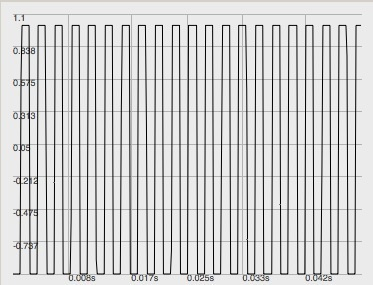
\includegraphics[width=5cm]{wv-impulse}
		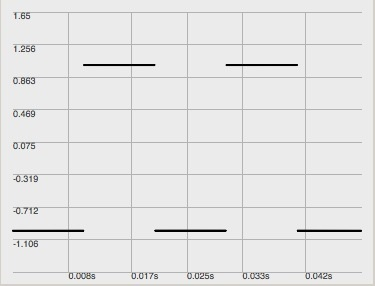
\includegraphics[width=5cm]{wv-pulse202}
		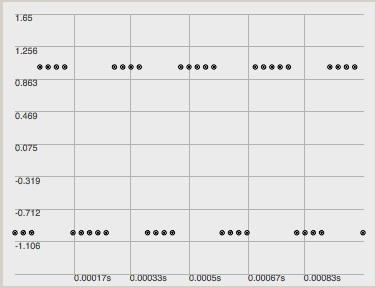
\includegraphics[width=5cm]{wv-pulse22}
		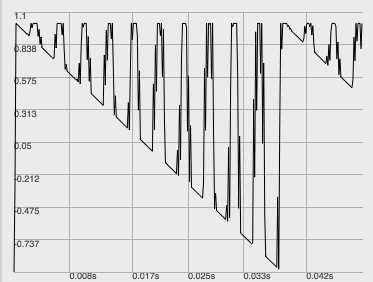
\includegraphics[width=5cm]{wv-sawImpulse}
		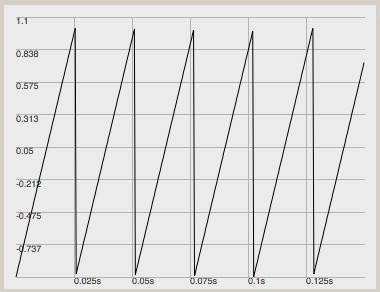
\includegraphics[width=5cm]{wv-sawtooth}
	\caption{Manually generated waveforms.}
	\label{fig:fig_waveforms_POPdestroy-random}
\end{figure}


%   + limitations and sonic characteristics of betablocker assembler programs
% TODO: find appropriate link to upper part
Findings: The shape of the waveform is limited due to the way the sound signal is derived from the Betablocker engine, namely probing the items on one of its functional parts, the stack. 
However, this limitation is inherent to the structure of the system itself.

\parskip 18pt

\subsubsection{Classic synthesis techniques adapted to Betablocker/Audio} % (fold)
\label{sub:classic_synthesis_techniques_adapted_to_betablocker}

Classic signal synthesis techniques such as additive synthesis, frequency modulation and amplitude modulation combine several sound generating modules in order to create new sounds.
The result depends highly on factors like the relation between the components, the signal characteristics of the base oscillators and the parameter range in which the oscillators control each other.

Next to being able to modulate its output amplitude, one feature of the Betablocker/Audio implementation in SuperCollider is that it allows to alter its calculation rate on a per-cycle basis.
This makes it possible to add dynamics not only in amplitude but also in pitch.
In several research-oriented livecoding sessions, we explored the sonic character of assembling Betablocker engines according to the mentioned classic synthesis techniques.

Figure~\ref{fig:classicSynthesisTechniquesFMAMAdditive} shows block diagrams for additive synthesis, frequency modulation and amplitude modulation of two  Betablocker/Audio modules.
While the implementation of these synthesis techniques is straight forward, the livecoding experimentation revealed several aspects worth mentioning:

% control-rate modulator
Adjusting the rate of the modulator in FM/AM synthesis to be below audio range results in sequencer-like monophonic synth patterns that are mostly pseudo-repetitive. 
I.e., they start with a chaotic movement that is followed by repetitions of a possibly slowly changing pattern.
This behaviour extends significantly the sonic qualities of a Betablocker/Audio engine, a feature Till used extensively in the livecoding performance at the SuperCollider symposium in London (see below report on Betablocker livecoding practice for details).

% audio-rate modulator
As known from classical FM synthesis, modulation rates in the audio range result in a broader frequency spectrum.
Linking the rates of all used Betablocker engines results in harmonic additions to the (noisy) spectra.
The sonic relation between different Betablocker programs seems to follow a specific rule, however, it is not a power of two relation.

% TODO interrelation between car and mod: sharing a buffer

% TODO wrap-up: allows for (limited) control of the output that can be used to induce musical structure on an otherwise uncontrolled behaviour (when playing with random heaps)

% FIXME should we add the listings of Additive/FM/AM, or maybe one of them as an example?

\begin{figure}
	\centering
		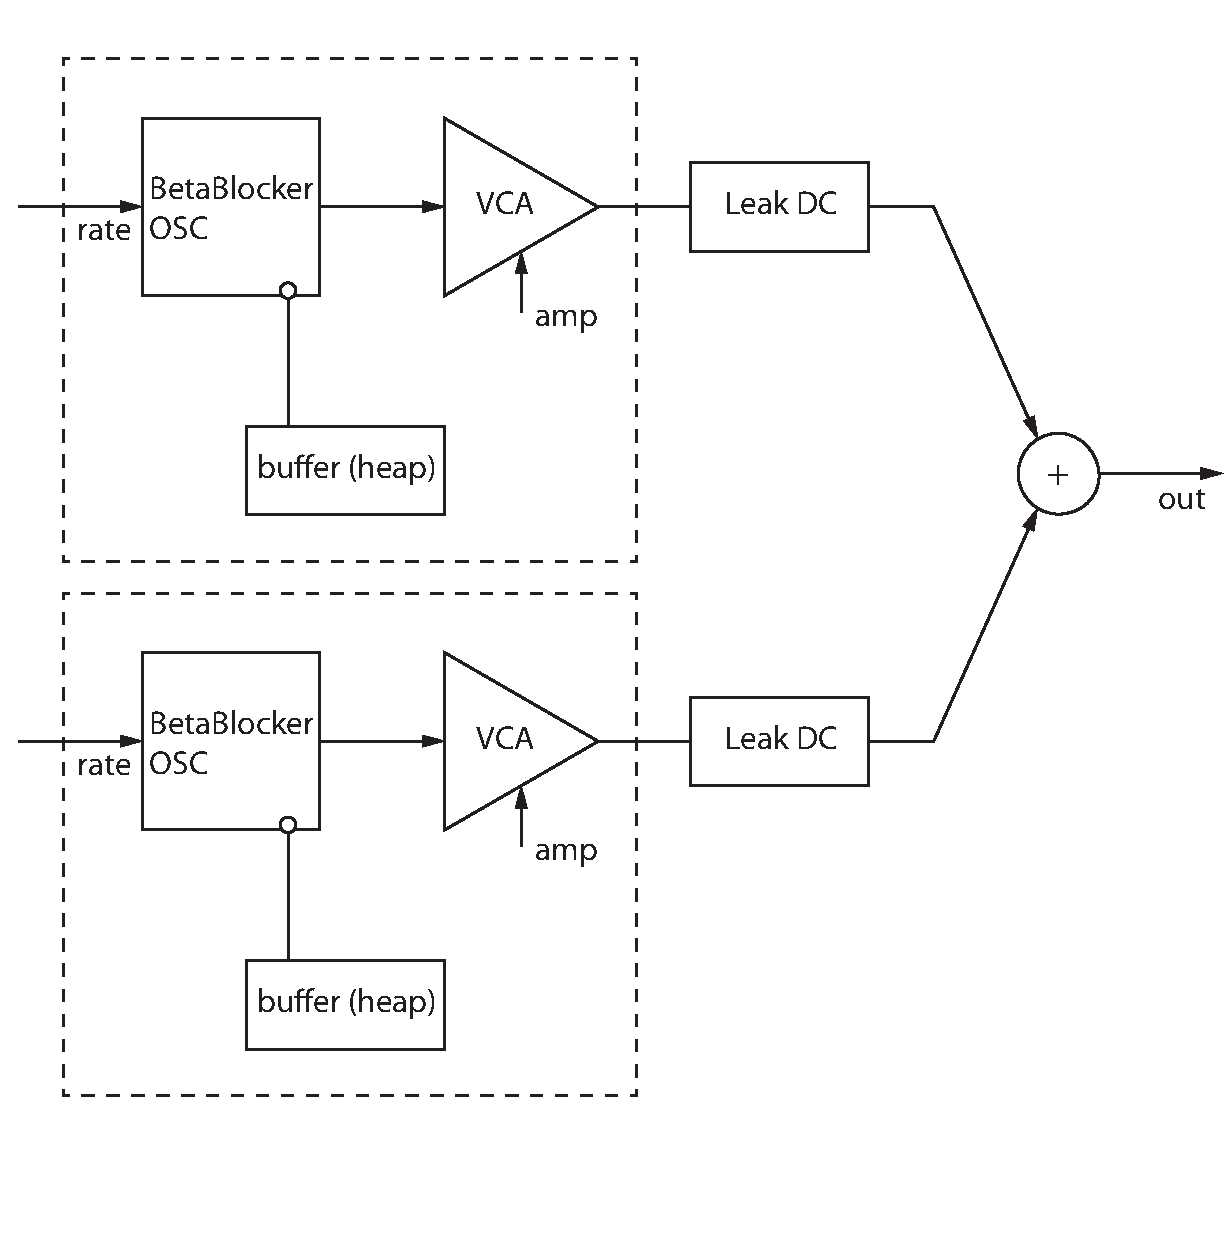
\includegraphics[height=4.5cm]{Additive-Betablocker}
		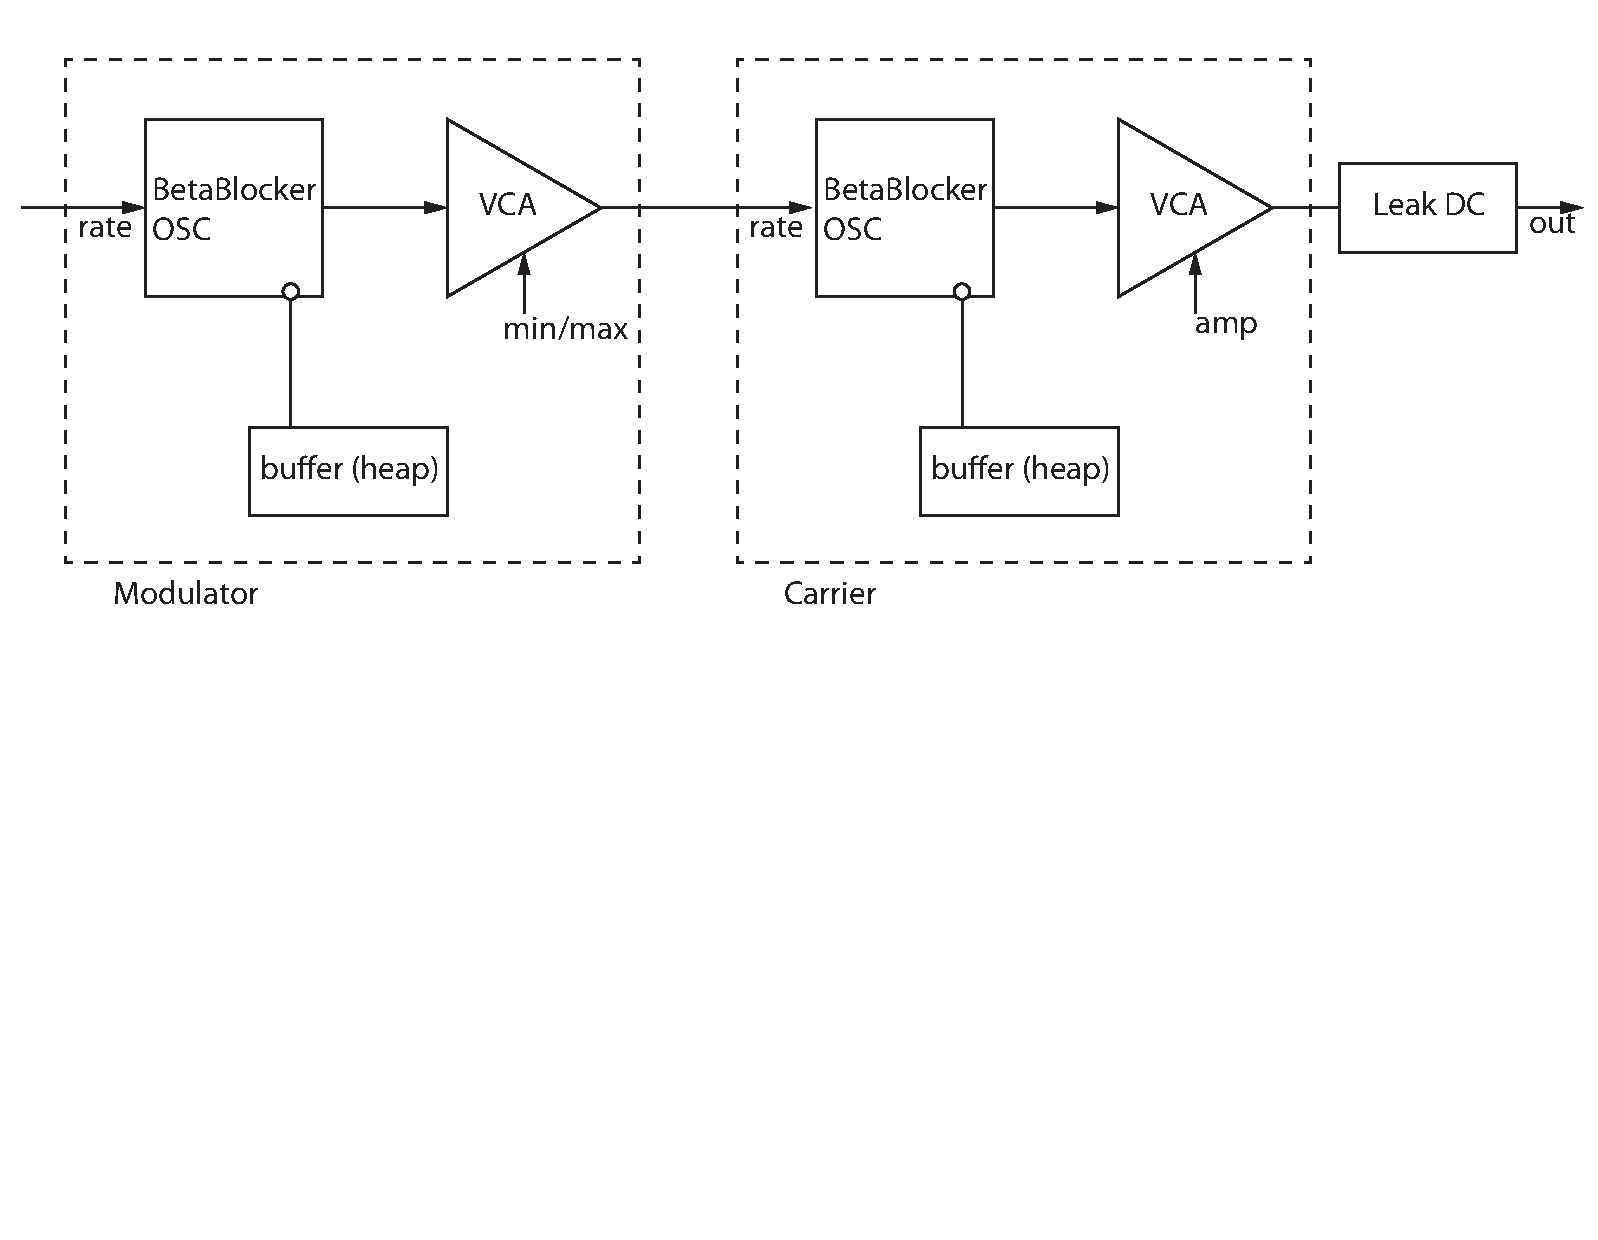
\includegraphics[height=4.5cm]{FM-Betablocker}
		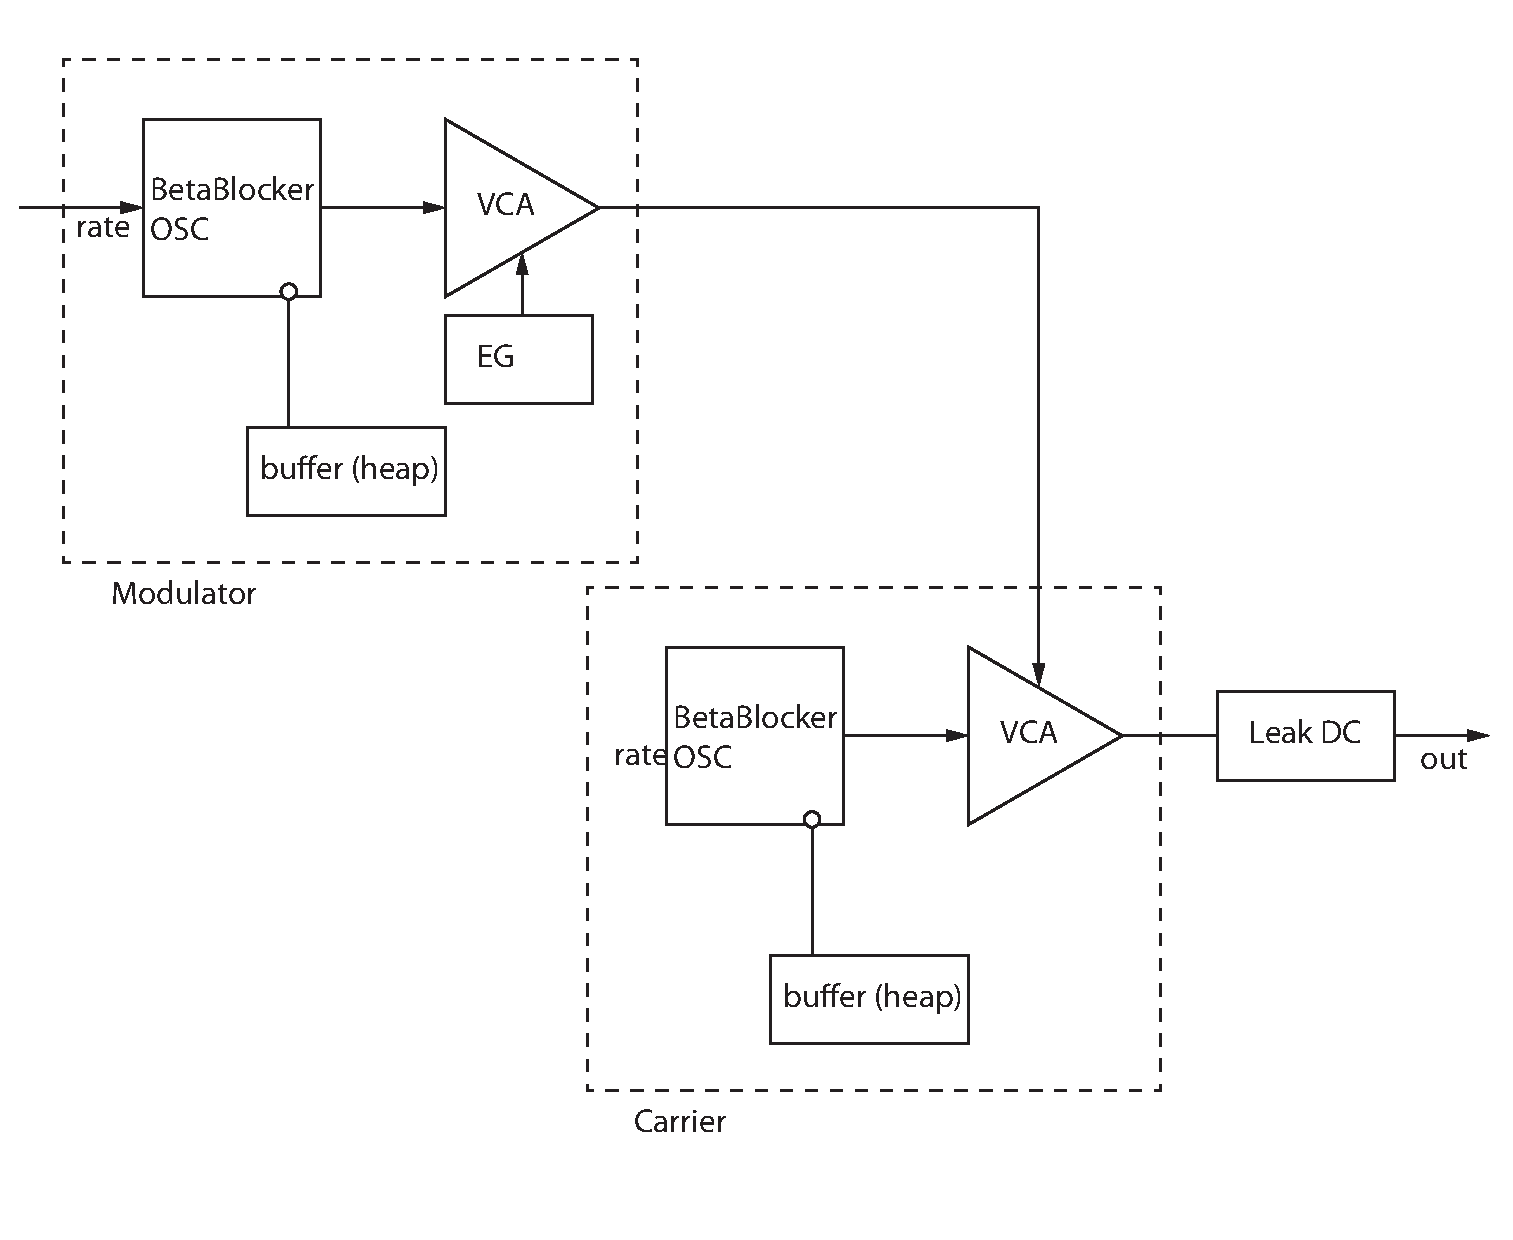
\includegraphics[height=4.5cm]{AM-Betablocker}
	\caption{Betablocker synthesis techniques.}
	\label{fig:classicSynthesisTechniquesFMAMAdditive}
\end{figure}

% Additive
% \begin{Verbatim}[fontfamily=courier, xleftmargin=\parindent]
% {var output, pC, stack;
% var numChains = 5;
% var ctls = ['rates'.kr(1000!numChains), 'bufnums'.kr(0!numChains), 'amps'.kr(0.1!numChains)].flop;
% 
% output = ctls.collect{|ctl|
%   # pC ... stack = BBlockerBuf.ar(
%     ctl[0], ctl[1]
%   );
%   LeakDC.ar(stack[0] * ctl[2]);
% };
% 
% Out.ar(0, output.sum)}.play;
% \end{Verbatim}
% 
% 
% FM:
% \begin{Verbatim}[fontfamily=courier, xleftmargin=\parindent]
% {var modulator, pC, stack, carrier;
% 
% modulator = Demand.ar(
%   Impulse.ar('modRate'.kr(2000)), 
%   'reset'.tr(0),
%   DetaBlockerBuf('modBufnum'.kr(0))
% ).linlin(-1, 1, 'modMinAmp'.kr(200), 'modMaxAmp'.kr(1600));
% 
% # pC ... stack = BBlockerBuf.ar(
% 	modulator, 'carBufnum'.kr(0)
% );
% carrier = LeakDC.ar(stack[0]);
% 
% Out.ar(0, carrier)}.play;
% \end{Verbatim}
% 
% 
% 
% AM:
% \begin{Verbatim}[fontfamily=courier, xleftmargin=\parindent]
% {var amp, pC, stack, output;
% 
% amp = Demand.ar(
%   Impulse.ar('modRate'.kr(2000)), 
%   'reset'.tr(0),
%   DetaBlockerBuf('modBufnum'.kr(0))
% ).linlin(-1, 1, 'modMinAmp'.kr(200), 'modMaxAmp'.kr(1600));
% 
% # pC ... stack = BBlockerBuf.ar(
%   'rate'.kr(1000), 'carBufnum'.kr(0)
% );
% output = LeakDC.ar(stack[0] * amp);
% 
% Out.ar(0, output)}.play;
% \end{Verbatim}


\parskip 18pt

\section{Betablocker and livecoding performance practice} 
\label{sec:betablocker_and_livecoding_practice_a_report}

Over the course of the last 3 years, we used Betablocker in a broad variety of livecoding practice, including both public performances and research-oriented investigations.
The result of the research process is reported in the above section.
Subsequent, we describe relevant Betablocker-based public performances in their order of appearance.

\parskip 18pt

\subsection{SuperCollider symposium London -- livecoding and visuals [4.2012]}
\label{sub:livecoding_and_visuals}

For the livecoding gig at the SuperCollider Symposium 2012, London, the two authors performed together for the first time. 
As they are not located at the same place, they developed a remote rehearsal routine in which each performer prepared his part as a sound recording and the other performed on top of it.
At the same time, both authors prepared their life sets.

Till's aesthetic goal for the performance was to play poly-rhythmical layers of coloured, noisy sounds with a setup purely based around his SuperCollider Betablocker implementation. 
At the same time, he aimed for a certain amount of transparency, i.e., it should be possible to not only see the changes he is making to the code but also how  Betablocker engines alter the heaps' content.
This meant 
(a) to develop a visual representation of the heaps he was playing, 
(b) to design a textual helper environment for his livecoding, mainly providing text blocks, and
(c) to pre-select heaps that he used as "raw materials" for his part of the  performance.

% TODO a visual language

\begin{figure}
	\centering
		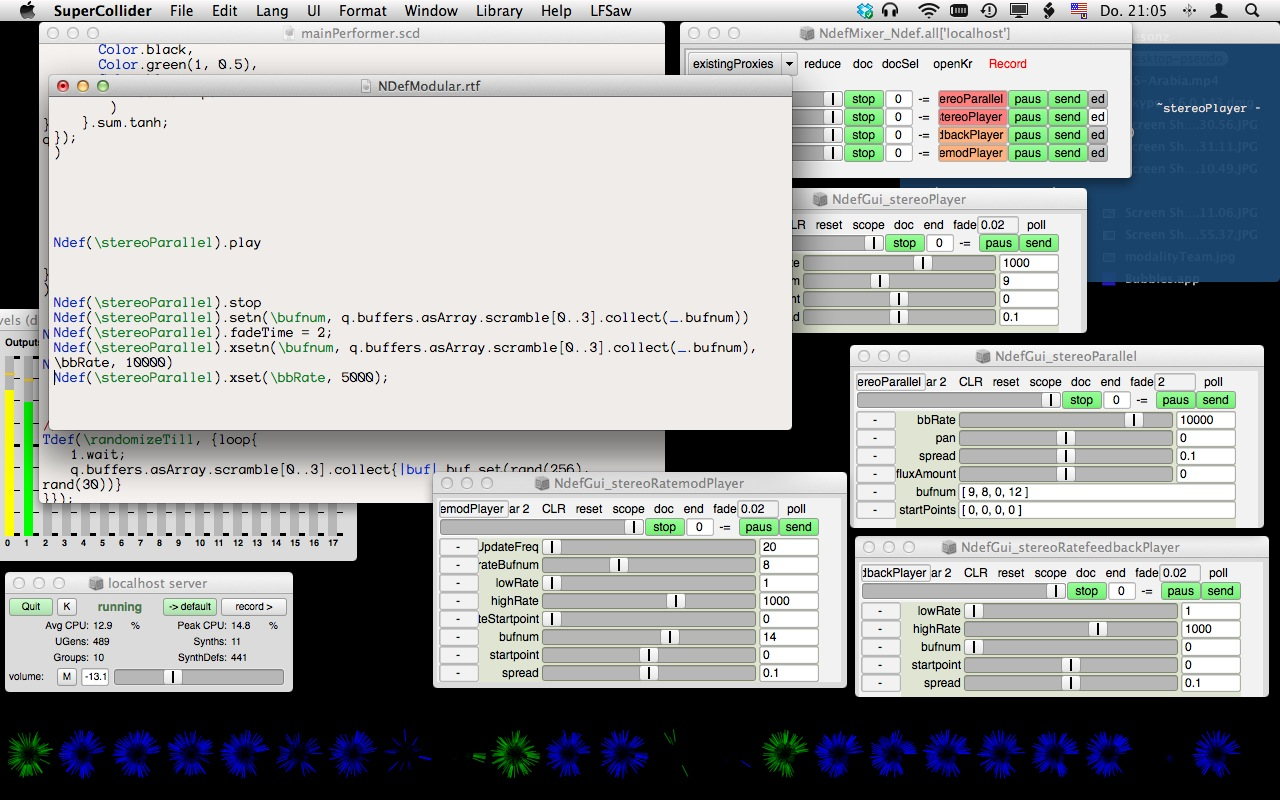
\includegraphics[width=10cm]{2012-SuperColliderSymposiumLiveCodingEnvironment-till}
	\caption{Till's livecoding environment as used at the SuperCollider symposium 2012, London.}
	\label{fig:fig_2012-SuperColliderSymposiumLiveCodingEnvironment-till}
\end{figure}


% \begin{figure}
% 	\centering
% 		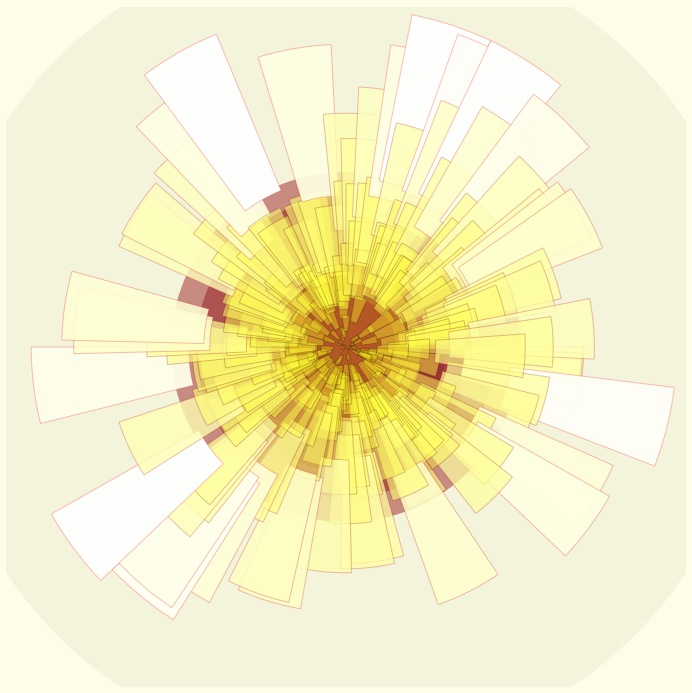
\includegraphics[width=5cm, height=5cm]{2013-heapIris-white}
% 		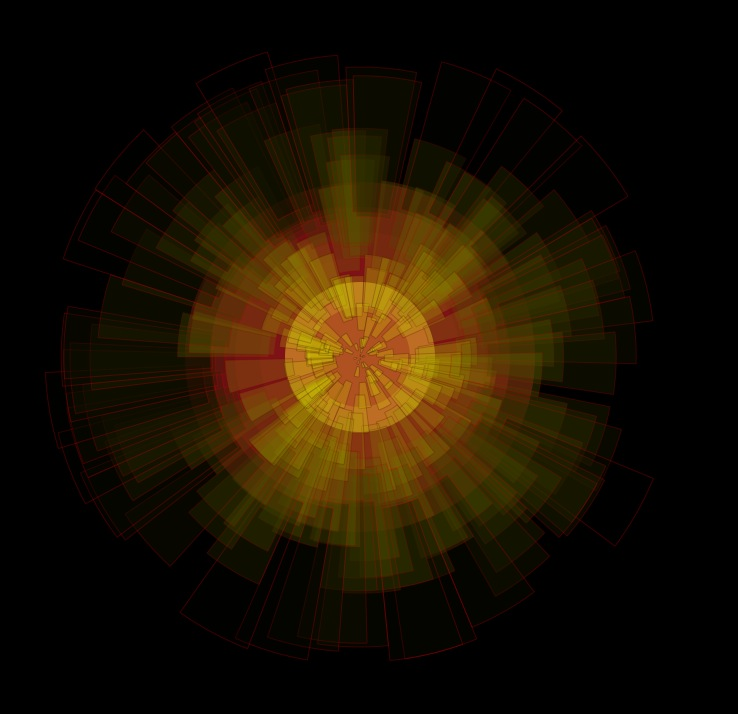
\includegraphics[width=5cm, height=5cm]{2013-heapIris-black}
% 	\caption{Iris-style visualisations of heaps.}
% 	\label{fig:fig_2013-heapIris-white}
% \end{figure}

Dave's aesthetic goal for the performance was to \dots
% TODO: dave describes his livecoding setup for the london performance

\parskip 18pt

\subsection{Oulipop -- translation of codes [5.2012, 4.2013]}
\label{sub:oulipop}

This piece for two performers and one laptop was conceptualised and realised by Till Bovermann and Sara Hildebrand Marques Lopes.
By manipulating texts according to Oulipo rules \citep*{mathews2005-oul}, it deals with the relation between writing and manipulating text, code and sound.

While editing text in one of two text panes, each keystroke also triggers a process that translates the current text's characters into a set of Betablocker/audio instructions. 
The correspondence of characters to instructions is defined by connecting the letter frequency for the performance language (here German) to values representing the influence of each instruction onto the rendered signal (e.g., \texttt{NOT} has a high value as it inverts the current output whereas \texttt{NOP} has a small value as it does not change the output).
Each line in the editor is treated as input to one Betablocker module.
The output of these Betablocker engines is organised in an FM-like structure. 
The resulting sound, an ever-changing blend of noisy texture and rhythmical patterns, influences the performers' decisions on how to further alter the text. 
Over the course of the performance, an initially meaningful text turns into nonsense before it eventually settles into a new and often surprising semantical meaning.\footnote{For more information and a documentation video, see \url{http://www.tai-studio.org/oulipop/}.}
\begin{figure}
	\centering
		\includegraphics[width=10cm]{20120509-IMG_3278}
	\caption{The Oulipop performance environment consists of a laptop with two typing areas.}
	\label{fig:fig_20120509-IMG_3278}
\end{figure}

\parskip 18pt

\section{Meta-Discussion}
\label{sec:meta}

% conclusions I think could be about the applicability over broad and general systems
% % fluxus/supercollider/gameboy ds/attiny

\parskip 18pt

\subsection{Explicit livecoding vs. meta-livecoding} 
\label{sub:explicit_livecoding_meta_livecoding}

% Explicit livecoding (here: on assembler level)
% meta-livecoding (here: the machine codes itself)

% listing about levels of livecoding possibilities with Betablocker

Livecoding with Betablocker can be done on various levels.
\begin{description}
	\item[Assembler-level programming] having full control over the program, apart of that it might modify itself at runtime, leading to
	\item[Self-modification] the engine itself modifies its heap and therefore its behavior
	\item[Structural programming] program interplay between several Betablocker engines (see also Section~\ref{sub:classic_synthesis_techniques_adapted_to_betablocker})
	\item[Amorphous/Genetic livecoding] determine intended machine output and have a genetic/learing algorithm solve that problem for you
\end{description}


\parskip 18pt

\subsection{Unfolding self modification to livecode pseudo-collaboration} 
\label{sec:unfolding_self_modification_to_livecode_collaboration}

Although the output of a given Betablocker stack is deterministic, it still is a mystery (i.e., not determinable) for the human mind - we want them to be like us so we suspend disbelief as a way to gain a tangible understanding

When working mostly with random data input, the pseudo-unpredicability kicks in quite heavily. 


% 
% \section{Appendix A}
% \label{sec:appendix_a}
% \begin{description}
% \item[\texttt{NOP}] do nothing
% \item[\texttt{ORG}] define relative origin address for this thread
% \item[\texttt{EQU}] compare first two elements on the stack, pop them off the stack, and push the result
% \item[\texttt{JMP}] jump to the address specified right after this instruction
% \item[\texttt{JMPZ}] jump only if stack returns 0
% \item[\texttt{PSHL}] push value on address specified right after this instruction to the stack
% \item[\texttt{PSH}] push value on address specified by the value on the address specified right after this instruction to the stack
% \item[\texttt{PSHI}] like push but one more encapsulation
% \item[\texttt{POP}] pop item from stack to the point in the heap following this instruction
% \item[\texttt{POPI}] pop item from stack and write the value at that address in the heap to the address following this instruction
% \item[\texttt{ADD}] perform an addition on the first two elements on the stack, pop them off the stack, and push the result
% \item[\texttt{SUB}] perform a subtraction on the first two elements on the stack, pop them off the stack, and push the result
% \item[\texttt{INC}] increment value on stack
% \item[\texttt{DEC}] decrement value on stack
% \item[\texttt{AND}] perform a bit-wise "and" on the first two elements on the stack, pop them off the stack, and push the result
% \item[\texttt{OR}] perform a bit-wise "or"" on the first two elements on the stack, pop them off the stack, and push the result
% \item[\texttt{XOR}] perform a bit-wise "xor" on the first two elements on the stack, pop them off the stack, and push the result
% \item[\texttt{NOT}] perform a bit-wise "not" on the first element on the stack, pop it off the stack, and push the result
% \item[\texttt{ROR}] perform a right shift operation on the first two elements on the stack, pop them off the stack, and push the result
% \item[\texttt{ROL}] perform a left shift operation on the first two elements on the stack, pop them off the stack, and push the result
% \item[\texttt{PIP}] increments value specified by the next value on the heap
% \item[\texttt{PDP}] decrements value specified by the next value on the heap
% \item[\texttt{DUP}] push a duplicate of the topmost value of the stack to the stack
% \item[\texttt{NOTE}] (DS extension) play a note
% \item[\texttt{VOX}] (DS extension) play a vox
% \item[\texttt{OUT}] (spork factory extension) pops the top of the stack and writes it to the pins on % \item[\texttt{STOP}] stop program (here: like NOP)
% an ATtiny
% \end{description}
% This is their actual implementation:
% 
% \begin{Verbatim}[fontfamily=courier, xleftmargin=\parindent]
% switch(instr)
% {
% case  NOP: break;
% case  ORG: m_start=m_start+m_pc-1; m_pc=1; break;
% case  EQU: push(pop()==pop()); break;
% case  JMP: m_pc=peek(m,m_pc++); break;
% case JMPZ: m_pc++; if (pop()==0) m_pc=peek(m,m_pc); break;
% case PSHL: push(peek(m,m_pc++)); break;
% case  PSH: push(peek(m,peek(m,m_pc++))); break;
% case PSHI: push(peek(m,peek(m,peek(m,m_pc++)))); break;
% case  POP: poke(m,peek(m,m_pc++),pop()); break;
% case POPI: poke(m,peek(m,peek(m,m_pc++)),pop()); break;
% case  ADD: push(pop()+pop()); break;
% case  SUB: push(pop()-pop()); break;
% case  INC: push(pop()+1); break;
% case  DEC: push(pop()-1); break;
% case  AND: push(pop()&pop()); break;
% case   OR: push(pop()|pop()); break;
% case  XOR: push(pop()^pop()); break;
% case  NOT: push(~pop()); break;
% case  ROR: push(pop()>>peek(m,m_pc++)); break;
% case  ROL: push(pop()<<peek(m,m_pc++)); break;
% case  PIP: 
% { u8 d=peek(m,m_pc++);
%   poke(m,d,peek(m,d)+1);
% } break;
% case  PDP:
% { u8 d=peek(m,m_pc++);
%   poke(m,d,peek(m,d)-1);
% } break;
% case  DUP: push(top()); break;
% default : break;
% };
% \end{Verbatim}
% 
% 
% \vspace*{24pt}
% 
% 
% 
% 
% 
% \vspace*{24pt}
% 

% % format for Heading-B style
% \subsection{Format for Heading-B Style; Use This for Subsection Headings}
% 
% Insert body text here.  
% 
% % format for Heading-C style
% \subsubsection{Format for Heading-C Style; Use This for Minor Sub-subsection Headings}
% 
% Insert body text here.
% 
% In the initial manuscript submission, you are encouraged to include figures (with captions) inline with the text, for ease of reading during the review process. For example, like this:
% 
% % include figures in text with captions for initial submission, like this:
% \begin{figure}[htpb]
% \begin{center}
% \includegraphics{myFigure.pdf}
% \caption{Insert Figure caption here.}
% \label{fig:myFigure}
% \end{center}
% \end{figure}
% 
% However, for the final version after the manuscript has been accepted, all figures should be moved to the end so that the text only contain markers like ``[Figure 1 about here]'' near where the figure would normally have occurred. You can rearrange the text to this effect simply by enabling the package {\tt endfloat} as suggested in the header of this document.
% 
% 
% % equations
% You can insert equations inline with the text like this:
% 
% \begin{equation}
% 	\label{radupdate}
% 		\Psi_{N}^{n+1} = m_{N}^{(-)}\Psi_{N-1}^{n}+m_{N}^{(0)}\Psi_{N}^{n} + q_{N}\Psi_{N}^{n-1}
% \end{equation}
% where
% \begin{eqnarray*}
% 	m_{N}^{(-)} &=& \frac{\lambda^2}{2\tau}\left(S_{N+1}+2S_{N}+S_{N-1}\right)\\
% 	m_{N}^{(0)} &=& \frac{1}{\tau}\left(2-\frac{\lambda^2}{2}\left(S_{N+1}+2S_{N}+S_{N-1}\right)\right)\\
% 	q_{N} &=& \frac{1}{\tau}\left(\frac{\gamma^2 k^2}{2h}\left(S_{N+1}+S_{N}\right)\left(\frac{\alpha_{1}}{k}-	\alpha_{2}\right)-1\right)
% \end{eqnarray*}
% and where 
% \begin{equation*}
% 	\tau = \frac{\gamma^2 k^2}{2h}\left(S_{N+1}+S_{N}\right)\left(\frac{\alpha_{1}}{k}+\alpha_{2}\right)+1
% \end{equation*}
% 
% % Use this environment for inserting source code examples.
% % Note, that this will print out text in the document exactly as you type it here in the .tex file. That means you can add empty spaces, tabs, blank lines here and they will be printed out like this in the document.). 
% %For more information check out the LaTeX-Package 'fancyvbr' documentation
% %
% \begin{Verbatim}[fontfamily=courier, xleftmargin=\parindent]
% Use this style for program code, for example:
% main() {
%     printf("Hello World\n");    
% }
% \end{Verbatim}
% 
% %use of references
% Some examples for the use of references in the text:\\
% %author name in sentence, single authors
% \cite{Ano08}, \cite{Bele68}, \cite{Ther99}, \cite{Zica02},
% %author name in sentence, multiple authors
% \cite*{VeRo00}, \cite*{AtDa04}, 
% %reference in brackets, multiple authors
% \citep*{AtDa04} 


%References
\bibliographystyle{cmj}
% \bibliography{cmjbib}
\bibliography{/Users/tboverma/Public/unpub/BibTeX/bovermann}
\end{document}
